\documentclass[11pt,a4paper]{article}
\usepackage[T1]{fontenc}
\usepackage[utf8]{inputenc}
\usepackage{lmodern,microtype,amsmath,amssymb,booktabs,enumitem}
\usepackage[margin=25mm]{geometry}
\usepackage{tikz}
\usetikzlibrary{arrows.meta,positioning,calc}
\usepackage{xcolor}
\usepackage{xurl}
\definecolor{darkred}{HTML}{8B0000}
\usepackage[colorlinks=true,linkcolor=darkred,urlcolor=darkred]{hyperref}
\setlength{\parindent}{0pt}
\setlength{\parskip}{7pt}
\renewcommand{\contentsname}{Indhold}
\renewcommand{\abstractname}{Resumé}
\setlist{nosep,leftmargin=*}
\title{A/B-forsøg med prisstrategier\\\large Præregistrering, økonomisk effekt og én slutanalyse}
\author{Danhostel Aarhus City · Prismotor}
\date{Metodeversion 1 · 17. oktober 2026}
\begin{document}
\maketitle
\begin{abstract}
Dette dokument beskriver den implementerede forsøgsmetode. A er den normale
prisstrategi, B er den fastlåste prismodel. V4 og V5 er varianter af samme model og er ikke
kontrolstrategien. Formålet er at estimere effekten af at tildele en prisstrategi på
faktisk dækningsbidrag pr. fysisk seng pr. nat. Et forsøg kræver prospektiv
randomisering, dokumenteret anvendelse og afstemte resultater. Prognosepræcision
og historiske korrelationer dokumenterer ikke denne effekt.
\end{abstract}
\tableofcontents
\newpage
\section{Spørgsmålet og forsøgets grænser}
Den videnskabelige inspiration er kontrollerede forsøg med en på forhånd valgt
Overall Evaluation Criterion (OEC), som beskrevet af Kohavi m.fl.\ [1]. Papiret
handler primært om værdien og kulturen omkring eksperimenter. Det foreskriver
ikke dette hostels blokdesign eller den konkrete inferens. Det følgende er en
lokal tilpasning; formlerne er beskrevet eksplicit.

Priser og kapacitet er fælles for gæsterne. Individuel lodtrækning pr. booking ville
kunne skabe konkurrence mellem forsøgsarmene om samme lager. Derfor anvendes
hele huset i blokke af \emph{opholdsdatoer}. Det er ikke et skift af strategi for alle
fremtidige datoer på én bestemt kalenderdag. Rumtyper og senge får samme arm på
en opholdsdato. Flerdagesophold henføres økonomisk til hver opholdsdato.

Gæster kan stadig flytte mellem datoer; bookinger kan krydse blokgrænser.
Randomisering fjerner ikke denne afsmitning. Betydelig afsmitning, ændrede
kanalvilkår eller anden samtidig behandling hindrer en simpel kausal fortolkning.
Bojinov m.fl.\ [3] viser netop, at carryover er et særskilt designproblem i
switchback-forsøg. Vi implementerer ikke deres optimale design eller deres
carryover-robuste estimator. Længere blokke kan mindske risikoen, men beviser
ikke, at den er væk. Vurdér opholdslængde, bookinghorisont og datofleksibilitet
før start; udfør først en driftsprøve med samme strategi i begge arme (A/A).

\begin{figure}[ht]
\centering\resizebox{.95\linewidth}{!}{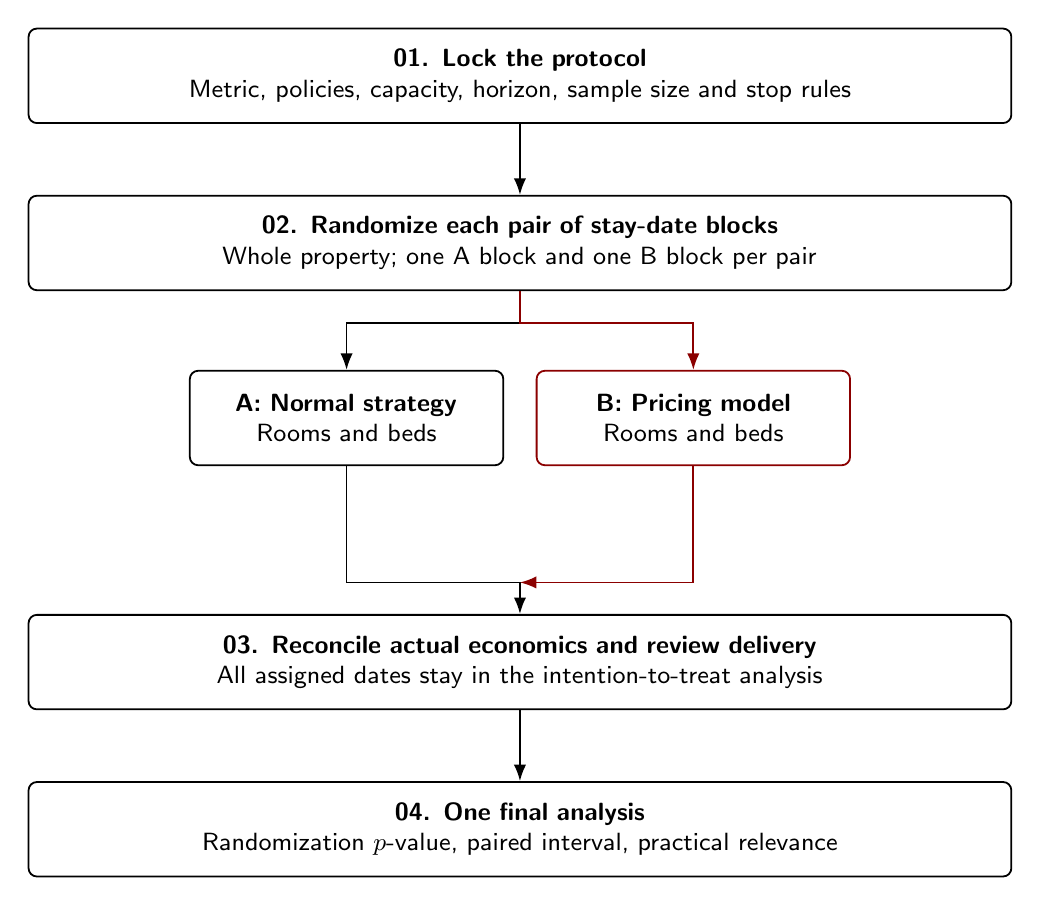
\begin{tikzpicture}[font=\sffamily\small,>=Latex,
 box/.style={draw=black,rounded corners=3pt,align=center,minimum height=12mm,text width=37mm,inner sep=4pt},
 every path/.style={line width=.65pt}]
\node[box,text width=122mm] (plan) {\textbf{01. Lock the protocol}\\Metric, policies, capacity, horizon, sample size and stop rules};
\node[box,below=9mm of plan,text width=122mm] (random) {\textbf{02. Randomize each pair of stay-date blocks}\\Whole property; one A block and one B block per pair};
\draw[->] (plan)--(random);
\node[box,below left=10mm and 2mm of random.south] (a) {\textbf{A: Normal strategy}\\Rooms and beds};
\node[box,below right=10mm and 2mm of random.south,draw=darkred] (b) {\textbf{B: Pricing model}\\Rooms and beds};
\draw[->] (random.south)--++(0,-4mm)-|(a.north);
\draw[->,darkred] (random.south)--++(0,-4mm)-|(b.north);
\node[box,below=41mm of random,text width=122mm] (out) {\textbf{03. Reconcile actual economics and review delivery}\\All assigned dates stay in the intention-to-treat analysis};
\draw[->] (a.south)|-($(out.north)+(0,4mm)$)--(out.north);
\draw[->,darkred] (b.south)|-($(out.north)+(0,4mm)$);
\node[box,below=9mm of out,text width=122mm] (final) {\textbf{04. One final analysis}\\Randomization $p$-value, paired interval, practical relevance};
\draw[->] (out)--(final);
\end{tikzpicture}
}
\caption{Fra låst protokol til låst resultat. Figuren viser designet, ikke indsamlede data.}
\end{figure}
\clearpage
\section{Præregistrering og tildeling}
Et par består af to på hinanden følgende lige lange blokke på $L\in\{7,14,28\}$
dage. Første blok starter mandag; ugedage er dermed repræsenteret ens i begge
arme. Hvert af $m$ par randomiseres uafhængigt med en fair mønt:
\begin{equation}
 Z_j\sim\operatorname{Bernoulli}(1/2),\qquad
 (T_{j1},T_{j2})=\begin{cases}(A,B)&Z_j=0,\\(B,A)&Z_j=1.\end{cases}
\end{equation}
Sæson og events er ikke identiske i to naboblokke. Randomisering håndterer dem i
forventning; få ekstreme datoer kan give stor usikkerhed. Alle grupper, events og
blokeringer indgår. Ingen datoer fjernes efter randomisering. Vil man afgrænse
en anden population, kræver det et nyt, foruddefineret design.

Før tildeling låses navn, A-strategiens konkrete regler, første dato, $m,L$,
fælles prisperiode $H$, fast fysisk kapacitet $C$, praktisk tærskel $\delta_\star$,
planlægningsspredning $\sigma_D$, stopregler og vurdering af afsmitning. Prisen
for hver opholdsdato styres efter sin arm fra $H$ dage før datoen til ankomst.
Første prisperiode skal begynde efter registreringsdagen. Allerede solgte ophold
omprissættes ikke. Deres resultat indgår i intention-to-treat (ITT), hvilket kan
fortynde effekten. Konklusionen gælder denne prisperiode og den valgte population.

Appen genererer en tilfældig seed, gemmer kalenderen og dens SHA-256-protokolhash.
En seed gør tildelingen reproducerbar; den er ikke bevis for korrekt prislevering.
Analysens kildekodehash og versionerne af NumPy og SciPy gemmes også. Ændringer
af dem blokerer en bekræftende slutanalyse med en anden metode end den registrerede.
Overlappende opholdsdatoer i registrerede forsøg afvises. Der er ingen redigering
eller ny lodtrækning i brugerfladen. JSON-eksporten indeholder protokol og log.

B's indlæste modelparametre, det aktuelle efterspørgselsniveau og centrale
kodefiler identificeres med hash. Den fælles online niveaulæring skal pauses
før registrering: resultater fra tidligere blokke kan ellers ændre senere
blokkes priser og skabe afsmitning via læringen. Teknisk kræves
\texttt{pricing.v4.level\_alpha: 0} og genindlæsning af konfigurationen.
Forsøgssektionen ændrer ikke selv indstillingen. Dette forsøg måler den
fastlåste politik; hele den adaptive politik kræver et andet design.
Genestimering af grundmodellen og ændringer af algoritme eller parametre er
en ny behandling. Nye markeds- og belægningsdata er tilladte input.
Appen kontrollerer aktuel hash ved slutanalyse; det er ikke en automatisk kontrol
af alle historiske tilstande. Blokgennemgangen skal dokumentere, at politikken
var stabil under hele forsøget. Forsøget skifter ikke automatisk priser i Picasso.

\section{Primært økonomisk mål}
For hver afsluttet opholdsdato $d$ anvendes:
\begin{align}
 G_d&=R_d^{\rm rum}+R_d^{\rm seng}+a_d-Q_d-V_d,\\
 Y_{jk}&=\frac{\sum_{d\in B_{jk}}G_d}{LC}.
\end{align}
$R$ er bogført logiomsætning eksklusive moms og morgenmad; $a_d$ er et eventuelt
ufordelt afstemt afrundingsbeløb; $Q_d$ er faktisk provision og $V_d$ faktisk
variabel omkostning på samme nettogrundlag og opholdsdato. Ukendte omkostninger
er manglende data, ikke nul. Modellens prisforslag er inklusive 25\% moms og
uden morgenmad; forslag indgår ikke som faktisk omsætning.

$C$ er det før forsøget fastlåste antal fysiske senge for hele huset, inklusive
senge i privatværelser. Det er ikke antal solgte senge, og flexkapacitet tælles
ikke dobbelt. Kapaciteten skifter ikke med B's allokering, belægning eller
blokeringer. Målet er derfor bidrag pr. \emph{fast fysisk seng pr. nat}, ikke det
øvrige dashboards RevPAB med faktisk tilgængelig kapacitet. Permanent ændret
kapacitet er et protokolbrud. Faste omkostninger indgår ikke; et højere bidrag er
ikke det samme som et dokumenteret højere regnskabsmæssigt overskud.

\section{Estimand og estimat}
Lad $Y_{jk}(B)$ og $Y_{jk}(A)$ være de potentielle blokresultater uden afsmitning.
Målet er den ligevægtede gennemsnitlige effekt over forsøgets $2m$ blokke:
\begin{equation}
 \tau=\frac{1}{2m}\sum_{j=1}^{m}\sum_{k=1}^{2}\{Y_{jk}(B)-Y_{jk}(A)\}.
\end{equation}
Hvert par leverer ét observeret bidragsestimat:
\begin{equation}
 D_j=Y_{j,B}^{\rm obs}-Y_{j,A}^{\rm obs},\qquad
 \widehat\tau=\bar D=\frac{1}{m}\sum_{j=1}^{m}D_j.
\end{equation}
Randomiseringen gør estimatet unbiased for $\tau$ under konsistens og ingen
afsmitning. Bookinger, prisberegninger og datoer inden for samme blok tæller
ikke som uafhængige forsøg. Afvigelser fra tildelt strategi bevares i den
oprindelige arm: ITT måler effekten af \emph{tildeling}, ikke en separat
effekt blandt dem, der faktisk fulgte strategien.

Den relative ændring vises deskriptivt som
$100\widehat\tau/\bar Y_A$ når $\bar Y_A>0$. Der gives ikke et separat
konfidensinterval eller en separat test for procenten. Antal solgte værelser og
senge vises hver for sig som sekundær beskrivelse uden nye hypotesetests.
\section{Én primær test og et omtrentligt interval}
\subsection{Randomiseringstest}
Den primære tosidede test anvender Fisher's \emph{skarpe nulhypotese}:
$H_0:Y_{jk}(B)=Y_{jk}(A)$ for alle blokke. Det er stærkere end blot
$\tau=0$; resultatet er ikke en eksakt test af den svage nulhypotese ved
heterogene effekter. Under den skarpe nulhypotese kan armene ombyttes uafhængigt
i hvert par. Med $T_{\rm obs}=|\sum_jD_j|$ fås
\begin{equation}
 p_{\rm exact}=2^{-m}\sum_{\epsilon\in\{-1,+1\}^{m}}
 \mathbf1\!\left\{\left|\sum_j\epsilon_jD_j\right|\ge T_{\rm obs}\right\}.
\end{equation}
Alle $2^m$ tildelinger gennemgås ved $m\le16$. Ved større $m$ trækkes
$M=99\,999$ tildelinger med en særskilt på forhånd gemt seed:
\begin{equation}
 p_{\rm MC}=\frac{1+\sum_{b=1}^{M}\mathbf1\{T_b\ge T_{\rm obs}\}}{M+1}.
\end{equation}
Plus-én-korrektionen [4] undgår et kunstigt $p=0$. Appen rapporterer metode og antal
træk. Flydende tal sammenlignes med en lille numerisk tolerance. Ved $m=6$ er
mindste eksakte tosidede $p$ omtrent $2/2^6=0.03125$; seks par er kun en teknisk
nedre grænse og ingen garanti for styrke.

\subsection{Parret interval}
Spredning og standardfejl beregnes som hos NIST [2]:
\begin{align}
 s_D^2&=\frac{1}{m-1}\sum_j(D_j-\bar D)^2,&
 \widehat{\operatorname{SE}}&=s_D/\sqrt m,\\
 I_{.95}&=\bar D\ \pm\ t_{.975,m-1}\,s_D/\sqrt m.
\end{align}
Intervallet er \emph{omtrentligt}, baseret på uafhængige par og en rimelig
normaltilnærmelse for pargennemsnittet; det er ikke inversion af
randomiseringstesten. Tidsmæssig afhængighed på tværs af par, få par eller meget
skæve/outlier-prægede bidrag kan gøre intervallet upålideligt. Ingen automatisk
winsorisering eller fjernelse af outliers udføres. Ved observeret nulspredning
vises intet interval, fordi et nulbredde-interval ville give falsk sikkerhed.

\subsection{Fortolkning og praktisk relevans}
$\alpha=0.05$ er låst og tosidet. Appen markerer positiv evidens når primær
$p\le0.05$ \emph{og} nedre omtrentlige intervalgrænse er over nul. En praktisk
relevant forbedring markeres først når grænsen også overstiger den forudvalgte
$\delta_\star$. Dette er en kombineret beslutningsregel, ikke en ny eksakt
randomiseringstest mod $\delta_\star$. Et usikkert resultat betyder ikke
ligeværdighed. $p$ er ikke sandsynligheden for, at modellen er bedre.

\begin{figure}[ht]
\centering\resizebox{\linewidth}{!}{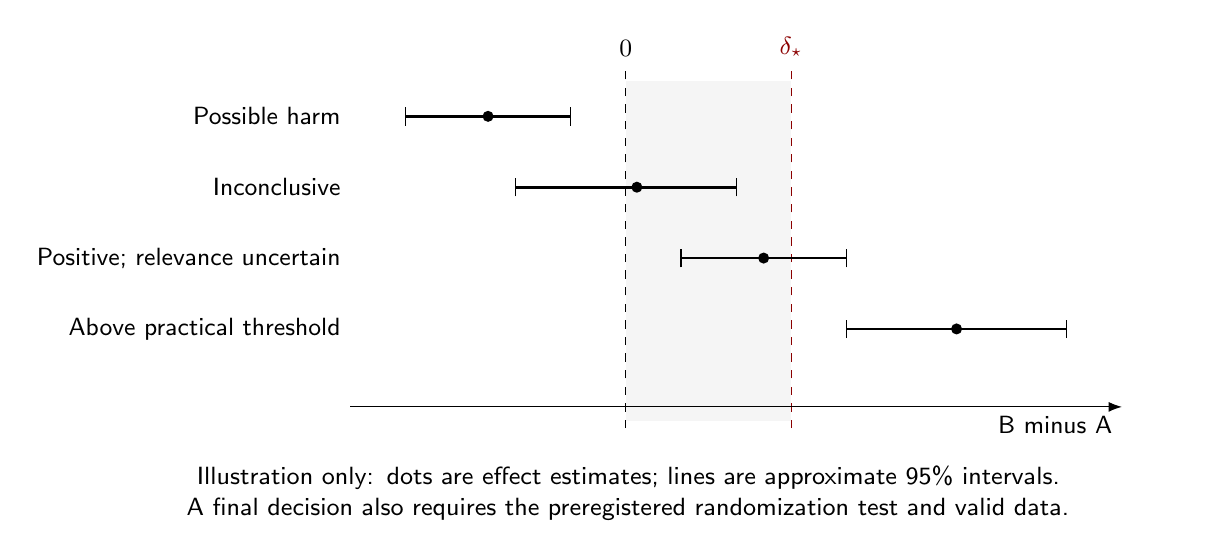
\begin{tikzpicture}[font=\sffamily\small,>=Latex,x=7mm,y=9mm]
\fill[black!4] (0,-.3) rectangle (3,4.5);
\draw[dashed] (0,-.4)--(0,4.7);
\draw[dashed,darkred] (3,-.4)--(3,4.7);
\node[above] at (0,4.7) {$0$};
\node[above,darkred] at (3,4.7) {$\delta_\star$};
\foreach \y/\l/\r/\m in {4/-4/-1/-2.5,3/-2/2/.2,2/1/4/2.5,1/4/8/6}{
 \draw[line width=1pt] (\l,\y)--(\r,\y);
 \draw (\l,\y-.13)--(\l,\y+.13);
 \draw (\r,\y-.13)--(\r,\y+.13);
 \fill (\m,\y) circle[radius=2pt];
}
\node[left,anchor=east] at (-5,4) {Possible harm};
\node[left,anchor=east] at (-5,3) {Inconclusive};
\node[left,anchor=east] at (-5,2) {Positive; relevance uncertain};
\node[left,anchor=east] at (-5,1) {Above practical threshold};
\draw[->] (-5,-.1)--(9,-.1) node[below left] {B minus A};
\node[align=center,text width=140mm,below] at (0,-.8) {Illustration only: dots are effect estimates; lines are approximate 95\% intervals.\\A final decision also requires the preregistered randomization test and valid data.};
\end{tikzpicture}
}
\caption{Illustrative intervaller; ingen af punkterne er faktiske forsøgsresultater.}
\end{figure}
\clearpage
\section{Styrke og varighed}
Det nødvendige antal par planlægges med en normaltilnærmelse:
\begin{equation}
 m_{\rm plan}=\max\left(6,\left\lceil
 \left[\frac{(z_{1-\alpha/2}+z_{1-\beta})\sigma_D}{\delta_\star}\right]^2
 \right\rceil\right),\qquad 1-\beta=0.80.
\end{equation}
$\sigma_D$ skal være spredningen af \emph{forskelle mellem parrede blokke}
i samme måleenhed som primærmålet. Det er ikke spredningen af daglig omsætning
eller individuelle bookinger. Estimér den fra sammenlignelige, afstemte
historiske økonomital eller en A/A-driftsprøve, og angiv begrundelsen i protokollen.

Eksempel: $\sigma_D=6$ og $\delta_\star=5$ kr. giver 12 par, altså 24 uger ved
$L=7$, plus mindst $H$ dages forløb og tid til regnskabsafstemning. Tallene er
illustrationer, ikke estimater fra hostellets data. Styrken er kun et skøn for et
parret middeltestdesign; den garanterer ikke 80\% styrke for den konkrete
randomiseringstest, især ved få par eller heterogene/skæve effekter. Brug en
forudgående designsimulation, hvis konklusionen kræver en præcis styrkegaranti.
Appen kræver mindst det omtrentlige planlægningsantal, men erstatter ikke dette arbejde.

\section{Drift, datakvalitet og låsning}
\begin{enumerate}
\item Beskriv A konkret: prisregler, informationsgrundlag, beslutningstidspunkt og
hvem der udfører dem. Hold kanaler, rabatter, minimumsophold, grupperegler og
andre indgreb fælles, medmindre de udtrykkeligt er en del af behandlingen.
\item Hent kalenderen. Anvend A/B for hver opholdsdato i den aftalte prisperiode.
Log anvendte priser og tidspunkt under Resultater. Gem bevis fra Picasso;
en CSV-eksport eller godkendelse beviser ikke anvendelse.
\item Registrér nye bookinger, annulleringer, manuelle indgreb, grupper,
blokeringer og events. Efter hver blok gemmes en driftsgennemgang med kilde og
afsløring af afvigelser. Rettelser til gennemgangen gemmes som nye logposter.
\item Importér og bekræft afsluttede resultater pr. opholdsdato; afstem logi
uden moms og morgenmad. Tilføj faktiske provisioner og variable omkostninger,
inklusive oplyst nul. En senere registrering, der tilbagekalder endelig status,
kan ikke ignoreres til fordel for en ældre komplet post.
\item Sluttest åbnes først, når alle planlagte datoer har fulde, bekræftede
resultater og alle blokke er gennemgået. Manglende data må hverken nuludfyldes
eller medføre selektiv fjernelse af par. Systemet viser datadækning undervejs,
men ingen inferentielle delresultater.
\item Før afslutning attesteres fælles regnskabsgrundlag, stabil behandling,
ingen væsentlig afsmitning og ingen selektion af datoer. Ved tvivl stoppes
forsøget som ugyldigt/ufuldstændigt, uden en bekræftende test. En attest er
operatørens vurdering og ikke et statistisk bevis for antagelserne.
\item Slutanalysen gemmer de præcise kildepost-ID'er, payloads, blokgennemgange,
protokolhash, tidspunkt og ansvarlig. Senere rettelser i resultatloggen ændrer
ikke dette snapshot. Fejl kræver en særskilt dokumenteret reanalyse, tydeligt
mærket som sådan; brugerfladen tilbyder ikke gentagne bekræftende analyser.
\end{enumerate}

Faste stopregler kan være prisfejl, gæsteklager, kapacitetsændring eller et
på forhånd aftalt driftsmæssigt tabskriterium. Appen overvåger dem ikke automatisk;
operatøren skal stoppe forsøget. En tidlig sikkerhedsstopning giver ingen
bekræftende $p$-værdi. Gentagen test indtil signifikans er ikke tilladt i denne
fast-horisont-metode. Eventuel sekventiel analyse kræver en ny metode/protokol.

Blokrandomiseringen garanterer præcis én A og én B pr. par. Et almindeligt
binomialt 50/50-SRM-test er derfor ikke relevant for antal blokke. Kontrollér i
stedet den gemte kalender, fuld datadækning og korrekt levering. Forskelle i
bookingantal er mulige behandlingseffekter og ikke i sig selv en tildelingsfejl.

Der er ét primært mål og én bekræftende test pr. protokol. Sekundære opdelinger
og procenttal er beskrivende. Gentagne eksperimenter på samme hypotese eller
valg af det bedste blandt mange kræver en samlet multiplicitetsplan;
appens enkelte protokol giver ikke automatisk kontrol af denne fejlrate.

\section{Hvad et positivt resultat kan sige}
Under designets antagelser giver et positivt resultat evidens for, at tildeling til
B øgede bidraget i den testede population og prisperiode. Det estimerer ikke
prisfølsomhed separat, garanterer ikke fremtidigt overskud og må ikke uden videre
omregnes til en årsgevinst. Resultater fra andre sæsoner, politikændringer og
større skala kræver opfølgning. Et A/A-forløb kontrollerer dataflow og drift;
et ikke-signifikant A/A-resultat beviser ikke fejlfrihed.

\section*{Referencer}
\addcontentsline{toc}{section}{Referencer}
\begin{enumerate}[label={[\arabic*]}]
\item Kohavi, R., Crook, T., Longbotham, R., Frasca, B., Henne, R., Lavista Ferres,
J. og Melamed, T. (2009). \emph{Online Experimentation at Microsoft}.
Brugerens offentlige ThinkWeek-version, især afsnit 2.
\url{https://www.microsoft.com/en-us/research/publication/online-experimentation-at-microsoft/}
\item NIST/SEMATECH. \emph{e-Handbook of Statistical Methods}, 7.3.1.1,
Analysis of paired observations.
\url{https://www.itl.nist.gov/div898/handbook/prc/section3/prc311.htm}
\item Bojinov, I., Simchi-Levi, D. og Zhao, J. \emph{Design and Analysis of
Switchback Experiments}. arXiv:2009.00148. Bruges til at belyse afsmitning;
deres estimator er ikke implementeret her.
\url{https://arxiv.org/abs/2009.00148}
\item Phipson, B. og Smyth, G. K. (2010). \emph{Permutation P-values Should
Never Be Zero: Calculating Exact P-values When Permutations Are Randomly Drawn}.
Statistical Applications in Genetics and Molecular Biology, 9(1), Article 39.
\url{https://doi.org/10.2202/1544-6115.1585}
\end{enumerate}
\end{document}
